\section{Measurements}
\label{sec:experiments:measurements}

Using the setup described in section \ref{sec:experiments:approach}, we have performed several experiments.

\begin{figure}[t]
	\centering
	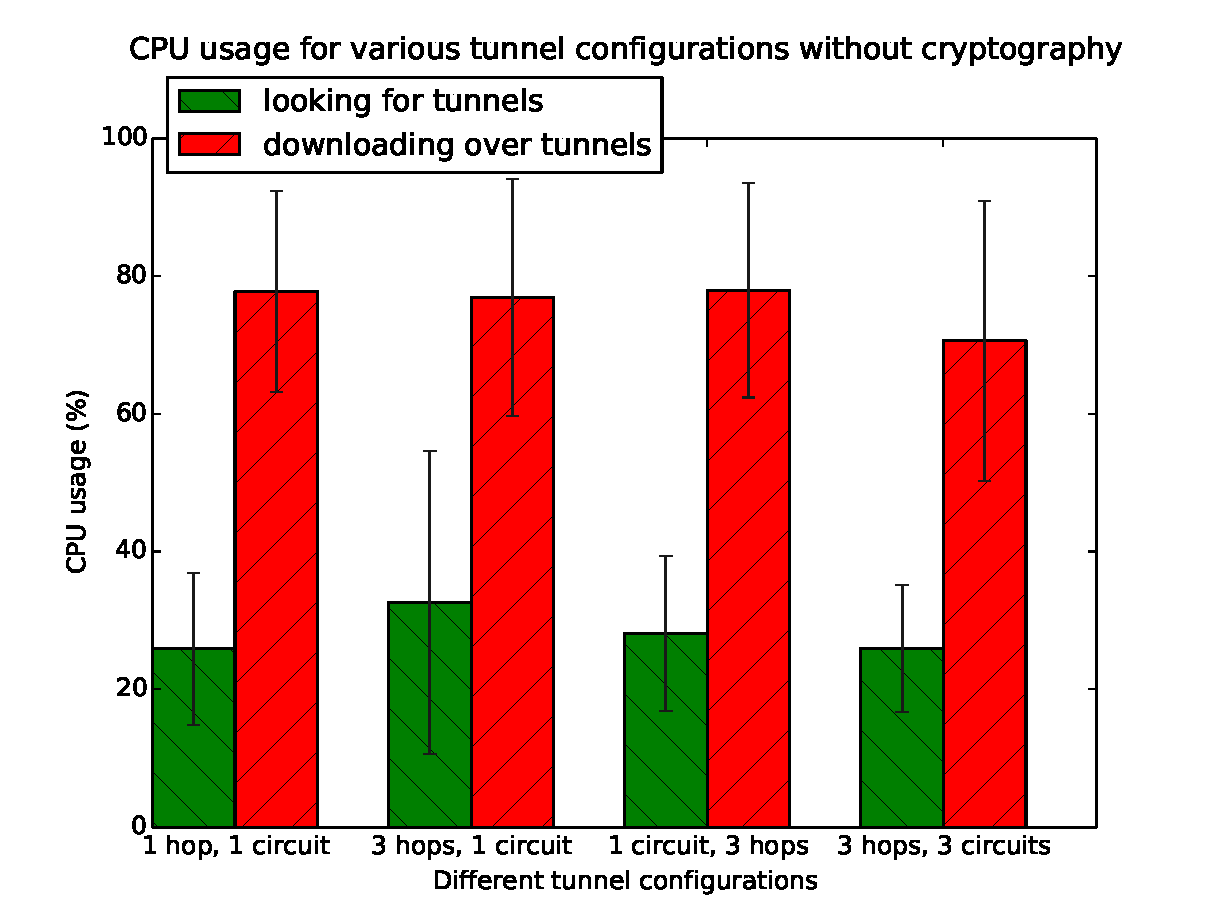
\includegraphics[width=0.85\textwidth]{graphics/cpu.pdf}
	\caption{CPU measurements for various tunnel configurations without cryptography.}
	\label{fig:cpu_measurements}
\end{figure}

By looking at the CPU usage we can determine whether running the anontunnels is too computationally expensive for the application of video streaming. Even without cryptography, we are seeing a CPU utilization of about 75\% when downloading (see Figure \ref{fig:cpu_measurements}). Due to the fact that we are not using cryptography, the amount of hops or circuits does not impact the CPU performance.

It is also interesting to look at the download speed of the application. This indicates whether we can accomplish the necessary bitrate to stream video, which is about 750 Kb/s (see Section \ref{sec:experiments:theoretical:bitrates}). We managed to achieve a download speed of around 500 - 600 KB/s on our test setup, which is sufficient for the application of video streaming (see Figure \ref{fig:download_measurements}). Due to the fact that all stand-alone anontunnels are running on the same computer, they will all perform equally well. Not a single one will act as a bottleneck. Additionally, the computer running the anontunnels is connected to the internet with a high speed connection of 100 Mb/s. Because of these factors, the amount of circuits or hops does not to matter. The computer is capable of relaying data fast enough to not impact the download speed of the Android device.

The time between when the download is triggered and when it actually receives its first byte is about 140 - 150 seconds when using 1 circuit. With 3 circuits, this takes about 180 - 190 seconds. This difference can be explained by the fact that more circuits take more time to setup.

\begin{figure}[t]
	\centering
	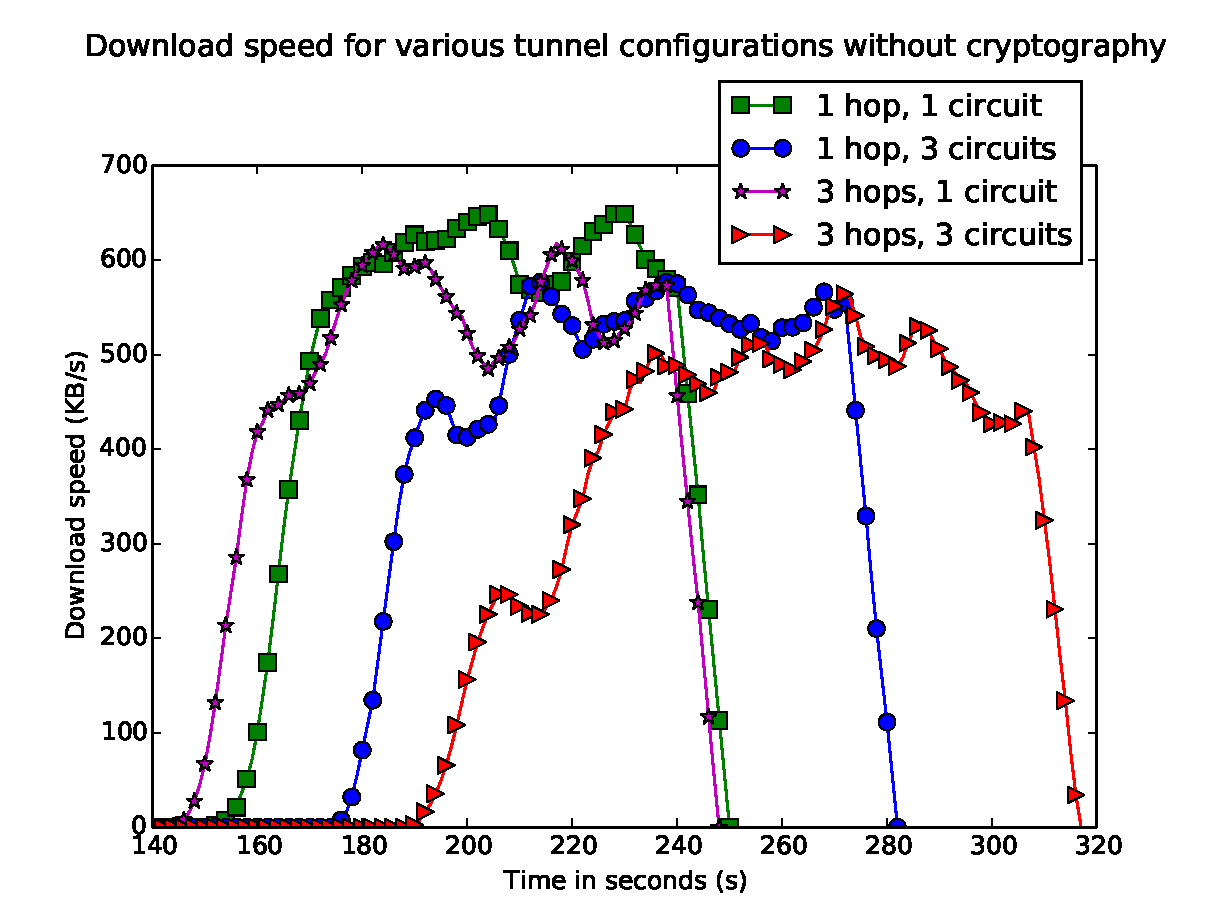
\includegraphics[width=0.85\textwidth]{graphics/downloadspeed.pdf}
	\caption{Download speed measured for various tunnel configurations without cryptography. The plot has been smoothed with a moving average of 10 seconds.}
	\label{fig:download_measurements}
\end{figure}
